\section{Minimum cut problem}

Let $G = (V, E)$ be a connected, undirected graph, where $n = \left\lvert V\right\rvert $ and $m = \left\lvert E\right\rvert $ represent the number of vertices and edges, respectively. 
For any subset $S \subset V$, the set $\delta(S) = \{(u, v) \in E \mid u \in S, v \in S^\prime\}$ defines a cut, separating the vertices in $S$ from those in $S^\prime=V\setminus S$. 
The minimum cut problem seeks to identify a cut with the fewest edges connecting $S$ and $S^\prime$, effectively partitioning the graph with minimal separation.

\subsection{Naive algorithm}
A traditional approach to solving the minimum cut problem is to compute $n-1$ minimum source-target cuts, one for each possible pair of vertices.
A source-target cut partitions the graph into two disjoint sets such that one subset contains a designated source vertex $s$ and the other contains a designated target vertex $t$.

The size of the minimum source-target cut is equivalent to the maximum flow between $s$ and $t$. 
The most efficient algorithm known for the maximum flow problem has a time complexity of:
\[T(n)=\mathcal{O}\left(nm \log\left(\frac{n^2}{m}\right)\right)\]
Here, $n$ is the number of vertices and $m$ is the number of edges. 

\subsection{Karger's algorithm}
Karger introduced a randomized algorithm that avoids explicit maximum flow calculations by using edge contraction to iteratively simplify the graph.
This contraction process preserves the minimum cut with high probability, resulting in a more efficient approach.

Edge contraction involves merging two vertices connected by an edge, $e=(u,v)$, into a single new vertex $w$. 
The contraction replaces all edges incident to $u$ or $v$ with edges incident to $w$, while removing any self-loops created by this merging process.
\begin{figure}[H]
    \centering
    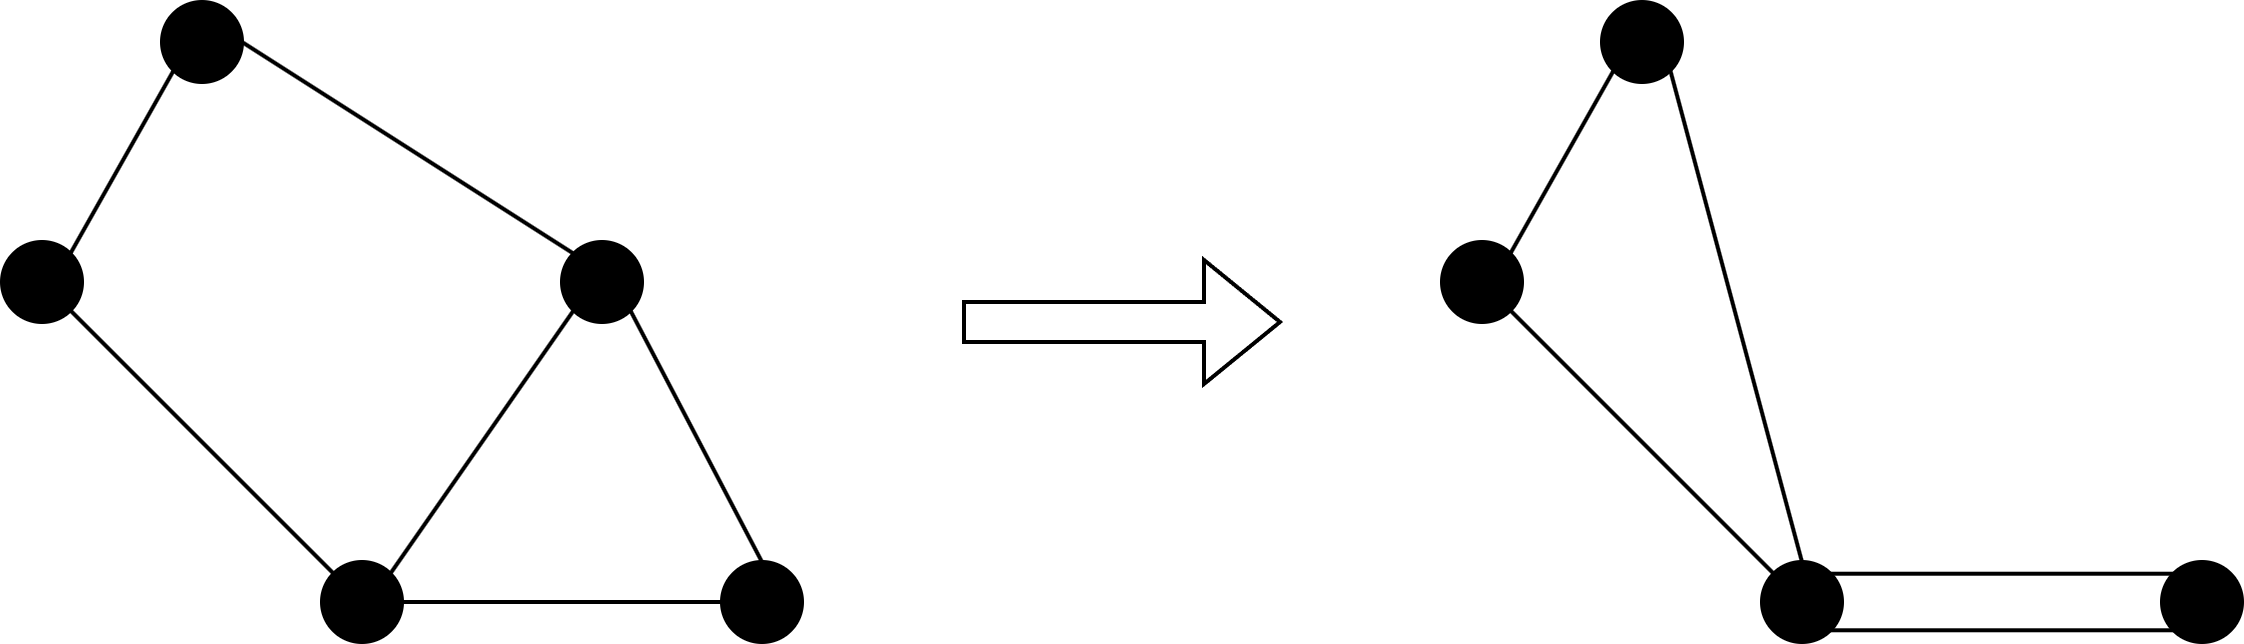
\includegraphics[width=0.8\linewidth]{images/ed.png}
    \caption{Edge contraction}
\end{figure}
\begin{definition}[\textit{Edge contraction}]
    For a multigraph $G=(V,E)$ without self-loops, contracting an edge $e=\{u,v\}\in E$, denoted $G\setminus e$, results in: 
\end{definition}
\begin{enumerate}
    \item Replacing vertices $u$ and $v$ with a new vertex $w$.
    \item Redirecting all edges incident to $u$ and $v$ to $w$. 
    \item Removing any self-loops involving $w$.
\end{enumerate}
After contraction, the graph $G\setminus e$ remains a multigraph.
Importantly, contracting $(u,v)$ does not affect cuts where $u$ and $v$ are both in the same set. 

\paragraph*{Algorithm}
Karger's algorithm for the minimum cut works as follows:
\begin{enumerate}
    \item Select an edge uniformly at random and contract its endpoints. 
    \item Repeat the contraction process until only two vertices remain.
\end{enumerate}
The two remaining vertices form a partition $(S, S^\prime)$ of the original graph, where the edges connecting $S$ and $S^\prime$ defines the cut $\delta(S)$ in $G$.
\begin{lemma}
    For a minimum cut $\delta(S)$ in the graph $G=(V,E)$, Karger's algorithm produces this minimum cut with probability at least:
    \[\Pr(\textnormal{minimum cut})\geq\dfrac{1}{\binom{n}{2}}\]
\end{lemma}
To increase the success probability, we repeat Karger's algorithm $l\cdot \binom{n}{2}$ times. 
The probability that at least one run will successfully produce the minimum cut is:
\[\Pr(\text{one success})\geq 1-e^l\]
Setting $l = c \log n$ reduces the error probability to less than:
\[\Pr(\text{error})\leq\dfrac{1}{n^c}\]

\paragraph*{Complexity}
One run of Karger's algorithm takes $\mathcal{O}(n^2)$ time.
By repeating the algorithm $\mathcal{O}(n^2\log n)$ times, we obtain a randomized algorithm with total time complexity:
\[T(n)=\mathcal{O}(n^4\log n)\] 

\subsection{Karger and Stein algorithm}
Karger and Stein refined Karger's original minimum cut algorithm to improve efficiency by enhancing the edge contraction process.
The core insight lies in understanding the telescoping product that emerges when calculating the probability of preserving edges in the minimum cut set $\delta(S)$ during contractions.

In the early stages, it's unlikely that an edge from the minimum cut set is contracted. 
However, as the graph reduces in size, the probability of contracting such an edge increases. 
By focusing on the probability that a fixed minimum cut $\delta(S)$ survives contraction to a subgraph with $l$ vertices, we find that:
\[\Pr(\text{cut survives})=\frac{\binom{l}{2}}{\binom{n}{2}}\]
Setting $l=\frac{n}{\sqrt{2}}$ ensures a survival probability of at least $\frac{1}{2}$.
This suggests that, on average, running two trials of the algorithm should be sufficient to find the minimum cut with high probability.

\paragraph*{Algorithm}
The Karger-Stein algorithm proceeds as follows for a multigraph $G$ with at least six vertices:
\begin{enumerate}
    \item Run the edge contraction algorithm on $\frac{n}{\sqrt{2}}+1$ vertices.
    \item Recur on the resulting contracted graph.
    \item Repeat these steps twice, then return the smaller of the two cuts found.
\end{enumerate}
Notably, setting the recursion threshold to six vertices affects only the constant factor of the runtime, without impacting the asymptotic complexity.
\begin{algorithm}[H]
    \caption{Karger and Stein}
    \begin{algorithmic}[1]
        \Function{contract}{$G=(V,E), t$}
            \While{$\left\lvert V\right\rvert  > t$}
                \State Choose $e\notin E$ uniformly at random
                \State $G=G\setminus e$
            \EndWhile 
            \State \Return $G$
        \EndFunction
        \Statex
        \Function{fastmincut}{$G= (V,E)$}
            \If {$\left\lvert V\right\rvert < 6$}
                \State \Return mincut($V$)
            \Else 
                \State $t= \left\lceil  1 + \frac{\left\lvert V\right\rvert}{\sqrt{2}}\right\rceil$
                \State $G_1 =$ \Call{contract}{$G, t$}
                \State $G_2 =$ \Call{contract}{$G, t$}
                \State \Return $\min \{$\Call{fastmincut}{$G_1$}, \Call{fastmincut}{$G_2$}$\}$
            \EndIf
        \EndFunction
    \end{algorithmic}
\end{algorithm}  

\paragraph*{Complexity}
The recurrence relation for the running time of the Karger-Stein algorithm is:
\[T(n) = T\left(\frac{n}{\sqrt{2}}\right) + \Theta(n^2)\]
Which solves to a complexity of $\mathcal{O}(n^2 \log n)$.

The algorithm's success probability at each recursive step is at least $\geq \frac{1}{2}$. 
To increase the probability of finding the minimum cut, we repeat the algorithm multiple times.
The probability of success is: 
\[\Pr(\text{success}) = \Omega\left(\dfrac{1}{\log n}\right)\]
Thus, to ensure the algorithm succeeds with high probability we need to run the algorithm $\mathcal{O}(\log^2 n)$ times. 
Thus, the total time complexity of the Karger-Stein algorithm is: 
\[T(n)=\mathcal{O}(n^2 \log^3 n)\]
\begin{corollary}
    Any graph has at most $\mathcal{O}(n^2)$ distinct minimum cuts.
\end{corollary}